\documentclass[titlepage]{article}

\usepackage[margin=1in]{geometry}
\usepackage{fancyhdr}
\usepackage{csquotes}
\usepackage{marginnote}
\usepackage{scrextend}
\usepackage[bottom]{footmisc}
\usepackage{enumitem}
\usepackage{amsmath,amssymb,amsthm}
\usepackage{mathtools,physics}
\usepackage{tikz,graphicx,subcaption}
\usepackage{pdfpages}
\usepackage[hidelinks]{hyperref}

\fancypagestyle{main}{
    \fancyhf{}
    \fancyhead[L]{\leftmark}
    \fancyhead[R]{MATH 16110}
    \fancyfoot[R]{Labalme \thepage}
}

\MakeOuterQuote{"}

\reversemarginpar

\deffootnotemark{\textsuperscript{\textup{[}\thefootnotemark\textup{]}}}
\deffootnote[2.1em]{0em}{0em}{\textsuperscript{\thefootnote}}

\setenumerate[itemize,3]{label={\scriptsize$\blacksquare$}}

\newcounter{script}

\newtheorem{lemma}{Lemma}
\newtheorem{corollary}{Corollary}
\newtheorem{theorem}{Theorem}[script]
\newtheorem{proposition}{Proposition}[script]
\newtheorem*{axioms}{Axioms}
\theoremstyle{definition}
\newtheorem{exercise}{Exercise}[script]

\usetikzlibrary{positioning,shapes}

\setcounter{secnumdepth}{0}

\newcommand{\N}{\mathbb{N}}
\newcommand{\Z}{\mathbb{Z}}

\title{MATH 16110 (Honors Calculus I IBL) Notes}
\author{Steven Labalme}

\begin{document}




\maketitle



\pagenumbering{roman}
\tableofcontents
\newpage



\pagenumbering{arabic}
\pagestyle{main}
\renewcommand{\sectionmark}[1]{\markboth{#1}{}}
\section{Introduction to Proofs}
\begin{itemize}
    \item \marginnote{9/27:}Note: These answers address the exercises on the following document.
    \item We will prove Lemma 4 (i) by contrapositive.
    \setcounter{lemma}{3}
    \begin{lemma}
        Let $x,y$ be positive integers. Then $xy$ is odd if and only if $x$ and $y$ are both odd.
        \begin{proof}
            We wish to prove that if $x$ and $y$ are not both odd, then $xy$ is not odd. In other words, we wish to prove that if at least one of $x$ or $y$ is even, then $xy$ is even. Let's begin. WLOG, let $x$ be even. Then $x=2k$ for some $k\in\N$. Thus, $xy=2(ky)$, proving that $xy$ is even since $ky\in\N$. The proof is symmetric for $y$.
        \end{proof}
    \end{lemma}
    \item We now prove Corollary 5.
    \setcounter{corollary}{4}
    \begin{corollary}
        Let $x,y$ be positive integers. Then $xy$ is even if and only if at least one of $x$ and $y$ is even.
        \begin{proof}
            We wish to prove that $xy$ is even if and only if at least one of $x$ and $y$ is even. Consequently, we must prove the dual implications "if $xy$ is even, then at least one of $x$ and $y$ is even" and "if at least one of $x$ and $y$ is even, then $xy$ is even." Let's begin. For the first statement, let $xy$ be even and suppose for the sake of contradiction that and both $x$ and $y$ are not even, i.e., are odd. But by Lemma 4, it follows from the assumption that $x$ and $y$ are both odd that $xy$ is odd, which contradicts the fact that $xy$ is even. Therefore, at least one of $x$ or $y$ must be even. As to the second statement, suppose that at least one of $x$ or $y$ is even. In this case, $x$ and $y$ are not both odd. Thus, by Lemma 4, $xy$ is not odd, or, equivalently, $xy$ is even.
        \end{proof}
    \end{corollary}
    \item Are there positive integers $m,n$ such that $m$ and $n$ have no common factors (other than 1) and $m^2=3n^2$? Either give an example or prove that no example is possible.
    \begin{proof}
        Let $m,n$ be relatively prime positive integers and suppose for the sake of contradiction that $m^2=3n^2$. We divide into two cases (the case where $n$ is even, and the case where $n$ is odd); we seek contradictions in both cases. First off, if $n$ is even, then $n=2k$ for some $k\in\N$. Thus, $3n^2=3(2k)^2=12k^2=2(6k^2)=m^2$, proving that $m^2$ is even since $6k^2\in\N$. By Corollary 5, this implies that $m$ is even. Therefore, since $m$ and $n$ are both even, they have a common factor, a contradiction. On the other hand, if $n$ is odd, then $n=2k+1$ for some $k\in\N$. Thus, $3n^2=3(2k+1)^2=12k^2+12k+3=2(6k^2+6k+1)+1=m^2$, proving that $m^2$ is odd since $6k^2+6k+1\in\N$. Thus, by Lemma 4, $m$ is odd. Consequently, $m=2l+1$ for some $l\in\N$, so $m^2=(2l+1)^2=4l^2+4l+1=12k^2+12k+3$, the last equality holding because we also have $m^2=3n^2=12k^2+12k+3$. This implies the following.
        \begin{align*}
            4l^2+4l+1 &= 12k^2+12k+3\\
            4l^2+4l &= 12k^2+12k+2\\
            2l^2+2l &= 6k^2+6k+1\\
            2(l^2+l) &= 2(3k^2+3k)+1
        \end{align*}
        Since $l^2+l$ and $3k^2+3k$ are both natural numbers, the above asserts that an odd number equals an even number, a contradiction. Hence, in both cases, we must have that $m^2\neq 3n^2$.
    \end{proof}
    \item Are there positive integers $m,n$ such that $m$ and $n$ have no common factors (other than 1) and $m^2=6n^2$? Either give an example or prove that no example is possible.
    \begin{proof}
        Let $m,n\in\N$ have no common factors (other than 1), and suppose for the sake of contradiction that $m^2=6n^2$. Since $m^2=6n^2=2(3n^2)$, $m^2$ is even. It follows by Corollary 5 that $m$ is even, implying that $m=2k$ for some $k\in\N$. Thus, $6n^2=m^2=(2k)^2=4k^2$, so $3n^2=2k^2$. Since $k^2\in\N$, $3n^2$ is even. Consequently, we have that $n^2$ is even by Corollary 5 (since at least one of 3 or $n^2$ is even and $3=2(1)+1$ is odd). By Corollary 5 again, $n$ is even. Thus, $m$ and $n$ are both even, contradicting the assumption that they have no common factors other than 1.
    \end{proof}
    \item Are there positive integers $m,n$ such that $m$ and $n$ have no common factors (other than 1) and $m^2=4n^2$? Either give an example or prove that no example is possible.
    \begin{proof}
        Let $m=2$ and $n=1$. Then $m^2=2^2=4=4\cdot 1^2=4n^2$.
    \end{proof}
\end{itemize}

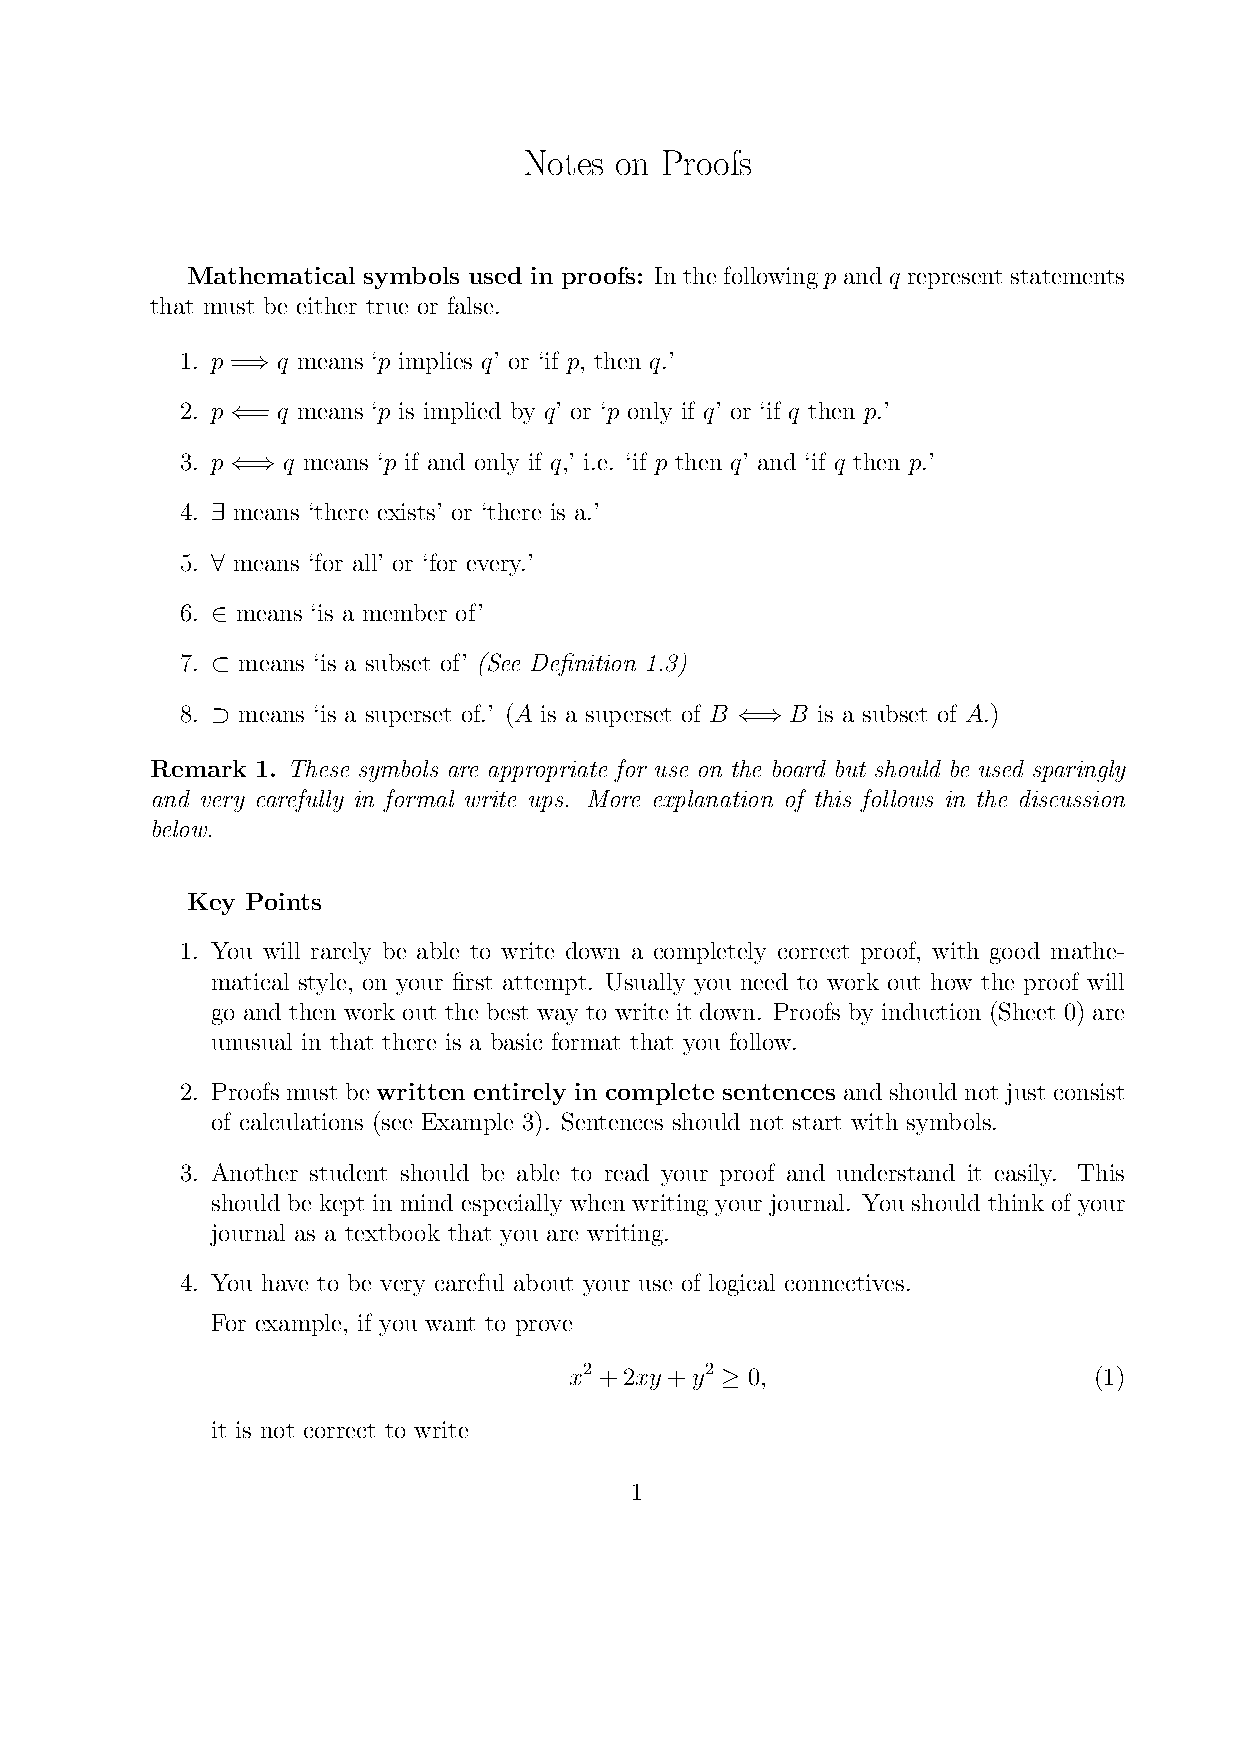
\includepdf[pages=-]{ExtFiles/WhatIsAMathematicalProof}



\section{Introduction to IBL}
\begin{itemize}
    \item \marginnote{9/29:}ZZ or zih-HWAY, Dixon Instructor in Department of Mathematics.
    \item Judson (super reader) is an advanced undergraduate who has taken this class before.
    \item Honors Calculus uses Spivak --- we do not have a textbook, just scripts!
    \begin{itemize}
        \item Few lectures in the traditional sense.
        \item Majority of material is presented and developed by the students.
        \item Several scripts will be covered throughout the quarter.
        \begin{itemize}
            \item In scripts: It is our job to complete the exercises, prove the theorems/lemmas/propositions, etc.
        \end{itemize}
        \item Be on the look-out for "\textcolor{green}{no proof required}" theorems.
        \item 3 chances to learn/review scripts material:
        \begin{enumerate}
            \item Before class, you prepare your own proof.
            \item During class, we discuss.
            \item After class and before the journal is due, we type up our own record of the proof in \LaTeX.
        \end{enumerate}
    \end{itemize}
    \item Before each class, she will tell us which theorems/exercises we need to work through.
    \item Your proofs do not have to be perfect in the beginning! Judson and ZZ will help us. Expect to present every other week.
    \begin{itemize}
        \item For the first two scripts, you have the ability to rewrite your journal after Judson reviews it to recover up to half of the lost credit.
        \item You only recover credit if your new solution is perfect.
        \item Return your changes one week after Judson grades it.
        \begin{itemize}
            \item Mark what parts/problems you have rewritten, and turn in the original as well.
        \end{itemize}
    \end{itemize}
    \item Later this afternoon, ZZ will share which Script 0 problems we should do before Thursday. Sign up for problems on a Google Sheet before 7:00 PM on Wednesday.
    \item She chooses a presenter based on our 0-3 rankings.
    \begin{itemize}
        \item A 0 means you don't know stuff or don't want to present.
        \item A 3 means you really want to present stuff.
        \item Other numbers are in between.
    \end{itemize}
    \item Class participation: When and how often and the quality of our presentations, and also how good are our questions that help presenters fill in the gaps.
    \item For hard proofs she may designate a backup presenter.
    \item We can use Overleaf for collaborative \LaTeX\ projects.
    \item We can check in with ZZ on our progress whenever throughout the quarter.
    \item She won't assign homework for the first week so that we can familiarize ourselves with \LaTeX.
    \begin{itemize}
        \item First HW assignment is due Thursday next week (10/8/2020)?
    \end{itemize}
    \item Judson's office hours: We get to talk to him one-on-one with questions.
    \begin{itemize}
        \item Problem session: we're all working collaboratively to figure something out.
    \end{itemize}
    \item You have one chance to ask for a 24-hour extension on HW (like if you're sick).
    \item In the case of a switch to virtual class:
    \begin{itemize}
        \item We can present by turning our phone into a document camera or using a white board behind us or typing up in \LaTeX\ (in real time?).
    \end{itemize}
    \item Get good at writing --- you cannot type up your solutions during exams!
    \item We submit HW assignments through Canvas if we type it up in \LaTeX, or in class by hand. It's nice if we can type it up.
\end{itemize}


\subsection{Problems}
\setcounter{exercise}{1}
\begin{exercise}[PMI Exercise 2]
    Prove that if $x>-1$, then $(1+x)^n\geq 1+nx$ for any natural number $n$. (Note that although this script is focused on the natural numbers, your argument should hold for any real number $x>-1$.)
    \begin{proof}
        We induct on $n$. For the base case $k=1$, we have $(1+x)^1=1+x\geq 1+(1)x$, where the greater than or equal to relation could be strengthened to equality but will be left as such for the sake of the argument. Now suppose inductively that we have proven the claim for some natural number $k$, i.e., we know that $(1+x)^k\geq 1+kx$ if $x>-1$. We now seek to prove it for $k+1$. To begin, we have
        \begin{align*}
            (1+x)^{k+1} &= (1+x)^k(1+x)
            \intertext{by the laws of exponents. By the inductive hypothesis and the fact that $ac\geq bc$ if and only if $a,b,c$ are positive numbers and $a\geq b$ (note that $x>-1$ implies $1+x>0$ along with $(1+x)^k>0$), we have that the above is}
            &\geq (1+kx)(1+x)
            \intertext{Now expand and simplify.}
            &= 1+kx+x+kx^2\\
            &= 1+(k+1)x+kx^2
            \intertext{Since $x^2$ must be positive or zero and $k\in\N$ is clearly positive, we have that $kx^2\geq 0$ so that the above is}
            &\geq 1+(k+1)x
        \end{align*}
        thus closing the induction.
    \end{proof}
\end{exercise}

\stepcounter{script}
\setcounter{theorem}{11}

\begin{theorem}
    Let $X$ be a set, and let $A,B\subset X$. Then
    \begin{enumerate}[label={\alph*\textup{)}}]
        \item $X\setminus(A\cup B)=(X\setminus A)\cap(X\setminus B)$
        \item $X\setminus(A\cap B)=(X\setminus A)\cup(X\setminus B)$
    \end{enumerate}
    \begin{proof}[Proof of a]
        To prove that $X\setminus(A\cup B)=(X\setminus A)\cap(X\setminus B)$, Definition 1.2 tells us that it will suffice to prove that $x\in X\setminus(A\cup B)$ if and only if $x\in (X\setminus A)\cap(X\setminus B)$, i.e., that if $x\in X\setminus(A\cup B)$, then $x\in (X\setminus A)\cap(X\setminus B)$ and if $x\in (X\setminus A)\cap(X\setminus B)$, then $x\in X\setminus(A\cup B)$. To begin, let $x\in X\setminus(A\cup B)$. By Definition 1.11, $x\in X$ and $x\notin A\cup B$. By Definition 1.5, it follows that $x\notin A$ and $x\notin B$. Since we know that $x\in X$ and $x\notin A$, Definition 1.11 tells us that $x\in X\setminus A$. Similarly, $x\in X\setminus B$. Since $x\in X\setminus A$ and $x\in X\setminus B$, we have by Definition 1.6 that $x\in(X\setminus A)\cap(X\setminus B)$, as desired. The proof of the other implication is the preceding proof "in reverse." For clarity, let $x\in(X\setminus A)\cap(X\setminus B)$. By Definition 1.6, $x\in X\setminus A$ and $x\in X\setminus B$. By consecutive applications of Definition 1.11, $x\in X$, $x\notin A$, and $x\notin B$. Since $x\notin A$ and $x\notin B$, Definition 1.5 reveals that $x\notin A\cup B$. But as previously established, $x\in X$, so Definition 1.11 tells us that $x\in X\setminus(A\cup B)$.
    \end{proof}
    \begin{proof}[Proof of b]
        To prove that $X\setminus(A\cap B)=(X\setminus A)\cup(X\setminus B)$, Definition 1.2 tells us that it will suffice to prove that $x\in X\setminus(A\cap B)$ if and only if $x\in (X\setminus A)\cup(X\setminus B)$. To begin, let $x\in X\setminus(A\cap B)$. By Definition 1.11, $x\in X$ and $x\notin A\cap B$. By Definition 1.6, it follows that $x\notin A$ or $x\notin B$. We divide into two cases. If $x\notin A$, then since we know that $x\in X$, Definition 1.11 tells us that $x\in X\setminus A$. It naturally follows that $x\in(X\setminus A)\cup(X\setminus B)$, since $x$ need only be an element of one of the two unionized sets (see Definition 1.5). The proof is symmetric if $x\notin B$. Now let $x\in(X\setminus A)\cup(X\setminus B)$. By Definition 1.5, $x\in X\setminus A$ or $x\in X\setminus B$. Once again, we divide into two cases. If $x\in X\setminus A$, then $x\in X$ and $x\notin A$ by Definition 1.11. Consequently, by Definition 1.6, $x\notin A\cap B$. Therefore, $x\in X\setminus(A\cap B)$ by Defintion 1.11. The proof is symmetric if $x\in X\setminus B$.
    \end{proof}
\end{theorem}

\setcounter{exercise}{18}

\begin{exercise}
    Must $f(f^{-1}(Y))=Y$ and $f^{-1}(f(X))=X$? For each, either prove that it always holds or give a counterexample.
    \begin{proof}
        We will address each statement in turn.\par
        Consider the sets $\{1\}$ and $\{3,4\}$, and let $f:\{1\}\to\{3,4\}$ be a function defined by $f(1)=3$. Let $Y=\{4\}$ (we clearly have $Y\subset\{3,4\}$ since 4 is the only element of $Y$ and $4\in\{3,4\}$ [see Definition 1.3]). Then $f^{-1}(Y)=\{a\in\{1\}\mid f(a)\in\{4\}\}=\emptyset$ and $f(f^{-1}(Y))=\{f(x)\in\{3,4\}\mid x\in\emptyset\}=\emptyset$ by consecutive applications of Definition 1.18. Therefore, $f(f^{-1}(Y))\neq Y$ since $4\in Y$ but $4\notin f(f^{-1}(Y))$ (see Definition 1.2)\footnote{Note that the reason $f(f^{-1}(Y))\neq Y$ in this case is because $f$ is not surjective.}.\par
        Similarly, consider the sets $\{1,2\}$ and $\{3\}$, and let $f:\{1,2\}\to\{3\}$ be a function defined by $f(1)=3$ and $f(2)=3$. Let $X=\{1\}$ (we clearly have $X\subset\{1,2\}$ since 1 is the only element of $X$ and $1\in\{1,2\}$ [see Definition 1.3]). Then $f(X)=\{f(x)\in\{3\}\mid x\in\{1\}\}=\{f(1)\}=\{3\}$ and $f^{-1}(f(X))=\{a\in\{1,2\}\mid f(a)\in\{3\}\}=\{1,2\}$ by consecutive applications of Definition 1.18. Therefore, $f^{-1}(f(X))\neq X$ since $2\in f^{-1}(f(X))$ but $2\notin X$ (see Definition 1.2)\footnote{Note that the reason $f^{-1}(f(X))\neq X$ in this case is because $f$ is not injective.}.
    \end{proof}
\end{exercise}

\setcounter{proposition}{25}

\begin{proposition}
    Let $A$, $B$, and $C$ be sets and suppose that $f:A\to B$ and $g:B\to C$. Then $g\circ f:A\to C$ and
    \begin{enumerate}[label={\alph*\textup{)}}]
        \item if $f$ and $g$ are both injections, so is $g\circ f$.
        \item if $f$ and $g$ are both surjections, so is $g\circ f$.
        \item if $f$ and $g$ are both bijections, so is $g\circ f$.
    \end{enumerate}
    \begin{proof}[Proof of a]
        Suppose that $(g\circ f)(a)=(g\circ f)(a')$. By Definition 1.25, this implies that $g(f(a))=g(f(a'))$. Since $g$ is injective, Definition 1.20 tells us that $f(a)=f(a')$. Similarly, the fact that $f$ is injective tells us that $a=a'$. Since we have shown that $(g\circ f)(a)=(g\circ f)(a')$ implies that $a=a'$ under the given conditions, we know by Definition 1.20 that $g\circ f$ is injective.
    \end{proof}
    \begin{proof}[Proof of b]
        Let $c$ be an arbitrary element of $C$. We wish to prove that there exists some $a\in A$ such that $(g\circ f)(a)=c$ (Definition 1.20). By Definition 1.25, it will suffice to show that there exists some $a\in A$ such that $g(f(a))=c$. Let's begin. By the surjectivity of $g$, there exists some $b\in B$ such that $g(b)=c$ (see Definition 1.20). If we now consider this $b$, we have by the surjectivity of $f$ that there exists some $a\in A$ such that $f(a)=b$ (see Definition 1.20). But this $a$ is an element of $A$ such that $g(f(a))=g(b)=c$, as desired.
    \end{proof}
    \begin{proof}[Proof of c]
        Suppose that $f$ and $g$ are two bijective functions. By Definition 1.20, this implies that $f$ and $g$ are both injections and are both surjections. Thus, by part (a), $g\circ f$ is an injection, and by part (b), $g\circ f$ is a surjection. Therefore, by Definition 1.20, $g\circ f$ is a bijection.
    \end{proof}
\end{proposition}



\section{Discussion of First Problem Set}
\begin{itemize}
    \item \marginnote{10/1:}See above for edits to my attempts for the proofs.
    \item Always make sure you use all given assumptions.
    \item $X\setminus A$ is the \textbf{complement} of $A$ (relative to $X$).
    \item We are allowed to assume that $x\in\{A:Q\}$ tells us that $x\in A$ and $Q$ is true? --- yes.
    \item We can let $x$ be an arbitrary element of a set and deduce stuff like in Tao.
    \item When we're writing proofs (consider Theorem 1.12), do we do not have to show the definition of $A\cap B$; we can just say "by Definition 1.6, $y\notin A\cap B$ implies that $y\notin a$ or $y\notin b$."
    \begin{figure}[h!]
        \centering
        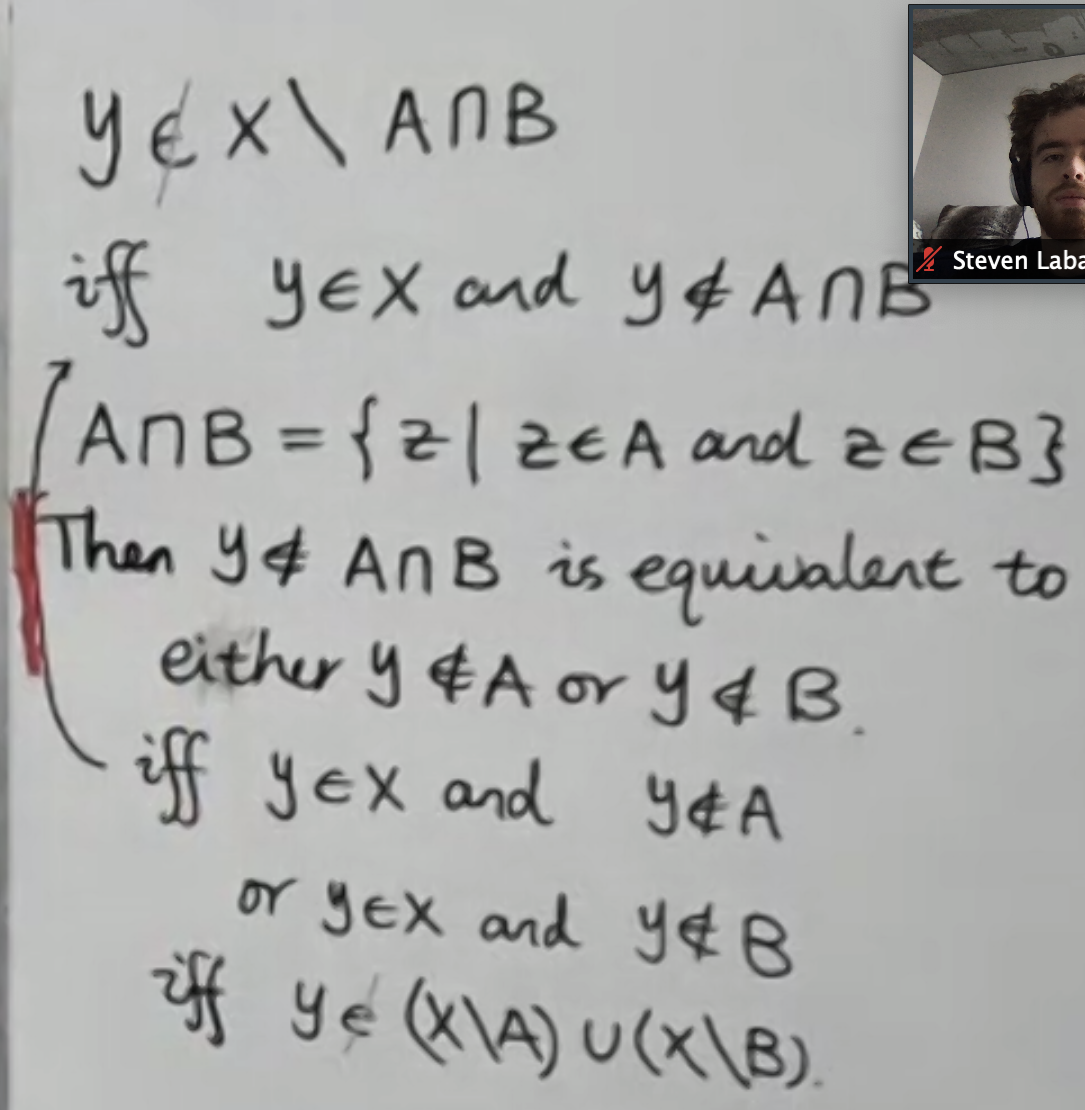
\includegraphics[width=0.3\linewidth]{ExtFiles/SampleTrm1-12Proof.png}
        \caption{Sample exam-ready proof of Theorem 1.12.}
        \label{fig:sampleTrm1-12Proof}
    \end{figure}
    \item What she wrote for the beginning of the proof of Theorem 1.12 (see Figure \ref{fig:sampleTrm1-12Proof}) is acceptable on an exam; in our exams, it will be the same as when presenting to class (we do not need complete sentences).
    \item Can we say "A similar argument works in reverse?"
\end{itemize}


\subsection{Problems}
\setcounter{exercise}{3}
\begin{exercise}
    Let $A=\{1,\{2\}\}$. Is $1\in A$? Is $2\in A$? Is $\{1\}\subset A$? Is $\{2\}\subset A$? Is $1\subset A$? Is $\{1\}\in A$? Is $\{2\}\in A$? Is $\{\{2\}\}\subset A$? Explain.
    \begin{proof}
        We list affirmative or negative answers and short explanations.\\[3pt]
        Yes, $1\in A$.\\
        No, $2\notin A$, but $\{2\}\in A$.\\
        Yes, $\{1\}\subset A$ since 1 is the only element of $\{1\}$ and $1\in A$ (as previously established).\\
        No, $\{2\}\not\subset A$ since $2\in\{2\}$ but $2\notin A$ (as previously established).\\
        No, $1\not\subset A$ since 1 is not a set.\\
        No, $\{1\}\notin A$, but $1\in A$ and $\{1\}\subset A$ as previously established.\\
        Yes, $\{2\}\in A$.\\
        Yes, $\{\{2\}\}\subset A$ since $\{2\}$ is the only element of $\{\{2\}\}$ and $\{2\}\in A$ (as previously established).
    \end{proof}
\end{exercise}

\setcounter{exercise}{9}

\begin{exercise}
    Show that if $A$ is any set, then $\emptyset\subset A$.
    \begin{proof}
        Suppose for the sake of contradiction that there exists a set $A$ such that $\emptyset\not\subset A$. Then by Definition 1.3, not every element of $\emptyset$ is also an element of $A$, i.e., there exists an element $x\in\emptyset$ such that $x\notin A$. But by Definition 1.8, $x$ (like all other objects) cannot be an element of $\emptyset$, a contradiction. Therefore, $\emptyset\subset A$ for all sets $A$.
    \end{proof}
\end{exercise}

\setcounter{exercise}{20}

\begin{exercise}
    Let $f:\N\to\N$ be defined by $f(n)=n^2$. Is $f$ injective? Is $f$ surjective?
    \begin{proof}
        $f$ is injective: Let $f(n)=f(n')$. Then $n^2=(n')^2$, implying that $n=n'$ (note that this last step is not permissible in all number systems, but it is within the naturals).\par
        $f$ is not surjective: For example, $2\in\N$ but there exists no natural number $n$ such that $f(n)=n^2=2$ (suppose for the sake of contradiction that there exists a natural number $n$ such that $n^2=2$. Since $n^2=2>1$, we know that $n<2$ (a number is less than its square if its square is greater than 1). But the only natural number less than 2 is 1, and $1^2=1\neq 2$, a contradiction).
    \end{proof}
\end{exercise}

\begin{exercise}
    Let $f:\N\to\N$ be defined by $f(n)=n+2$. Is $f$ injective? Is $f$ surjective?
    \begin{proof}
        $f$ is injective: Let $f(n)=f(n')$. Then $n+2=n'+2$, implying by the cancellation law for addition that $n=n'$.\par
        $f$ is not surjective: For example, $1\in\N$ but there exists no natural number $n$ such that $n+2=1$ (suppose for the sake of contradiction that there exists a natural number $n$ such that $n+2=1$. Because $1=n+2$, we know that $1>n$. But we also know that $1\leq n$ for all $n\in\N$ (as can be proven by induction), which contradicts the trichotomy).
    \end{proof}
\end{exercise}

\begin{exercise}
    Let $f:\Z\to\Z$ be defined by $f(x)=x^2$. Is $f$ injective? Is $f$ surjective?
    \begin{proof}
        $f$ is not injective: For example, $f(2)=4=f(-2)$, but $2\neq -2$.\par
        $f$ is not surjective: For example, $2\in\Z$ but there exists no integer $x$ such that $f(x)=x^2=2$ (suppose for the sake of contradiction that there exists an integer $x$ such that $x^2=2$. Since $x^2=2$, $|x|<2$ for similar reasons to those discussed in Exercise 1.21. Thus, $x=-1$, $x=0$, or $x=1$. But $(-1)^2=1\neq 2$, $0^2=0\neq 2$, and $1^2=1\neq 2$, a contradiction).
    \end{proof}
\end{exercise}

\setcounter{proposition}{26}

\begin{proposition}
    Suppose that $f:A\to B$ is bijective. Then there exists a bijection $g:B\to A$ that satisfies $(g\circ f)(a)=a$ for all $a\in A$, and $(f\circ g)(b)=b$ for all $b\in B$.
    \begin{proof}
        Let $g:B\to A$ be defined by the rule, "$g(b)=a$ if and only if $f(a)=b$." For $g$ to be a function as defined, Definition 1.16 tells us that we must show that for every $b\in B$, there exists a unique $a\in A$ such that $g(b)=a$. By the surjectivity of $f$, we know that for all $b\in B$, there exists \emph{an} $a\in A$ such that $f(a)=b$. On the uniqueness of this $a$, let $a\neq a'$ and suppose for the sake of contradiction that $g(b)=a$ and $g(b)=a'$. By the definition of $g$, we have that $f(a)=b$ and $f(a')=b$, so $f(a)=f(a')$. But by the injectivity of $f$, this means that $a=a'$, a contradiction. Therefore, $g$ indeed maps every $b\in B$ to a unique $a\in A$. To demonstrate that $g$ satisfies the remainder of the necessary constraints, we will work through them one by one.\par
        To prove that $g$ is injective, Definition 1.20 tells us that we must verify that if $g(b)=g(b')$, then $b=b'$. Let $g(b)=g(b')$. Since $g$ is a function, $g(b)=g(b')=a$, where $a\in A$. This implies by the definition of $g$ that $f(a)=b$ and $f(a)=b'$. But this means that $b=f(a)=b'$, as desired. To prove that $g$ is surjective, Definition 1.20 tells us that we must verify that for all $a\in A$, there exists a $b\in B$ such that $g(b)=a$. Let $a$ be an arbitrary element of $A$. By Definition 1.16 and the status of $f$ as a function, there exists an element $b\in B$ such that $f(a)=b$. But by the definition of $g$, $f(a)=b$ implies that $g(b)=a$, meaning that this $b$ satisfies the desired constraint. On the basis of this and the previous argument, Definition 1.20 allows us to conclude that $g$ is bijective.\par
        We now prove that $(g\circ f)(a)=a$ for all $a\in A$. Let $a$ be an arbitrary element of $A$. Then by Definition 1.16 and the status of $f$ as a function, $f(a)=b$ where $b\in B$. Thus, by the definition of $g$, $g(b)=a$, implying that $g(b)=g(f(a))=a$. But by Definition 1.25, $g(f(a))=(g\circ f)(a)=a$, as desired.\par
        A symmetric argument can demonstrate that $(f\circ g)(b)=b$ for all $b\in B$.
    \end{proof}
\end{proposition}

\setcounter{theorem}{31}

\begin{theorem}
    Let $A$ be a finite set. Suppose that $A$ is in bijective correspondence both with $[m]$ and with $[n]$. Then $m=n$.
    \begin{proof}
        If $A$ is in bijective correspondence with both $[m]$ and with $[n]$, then Definition 1.28 tells us that there exist bijections $f:[m]\to A$ and $g:A\to[n]$. Thus, by Proposition 1.26, $g\circ f:[m]\to[n]$ is bijective. Now suppose for the sake of contradiction that $m\neq n$. Then by the trichotomy, either $m>n$ or $m<n$. We divide into two cases. If $m>n$, then Theorem 1.31 tells us that no injective function $h:[m]\to[n]$ exists. But $f:[m]\to[n]$ is bijective, hence injective by Definition 1.20, a contradiction. On the other hand, if $m<n$, then Theorem 1.31 tells us that no injective function $h:[n]\to[m]$ exists. But by Proposition 1.27, the existence of the bijection $f:[m]\to[n]$ implies the existence of a bijection $f^{-1}:[n]\to[m]$. As before, the bijectivity of $f^{-1}$ implies that it is also injective by Definition 1.20, a contradiction. Therefore, we must have $m=n$ based on the given conditions. 
    \end{proof}
\end{theorem}

\noindent\textbf{Additional Exercises}
\begin{enumerate}
    \item In each of the following, write out the elements of the sets.
    \begin{enumerate}
        \item[a)] $(\{n\in\Z\mid n\text{ is divisible by }2\}\cap\N)\cup\{-5\}$
        \begin{proof}
            The elements are $-5$ as well as 2, 4, 6, and every other even natural number.
        \end{proof}
        \item[c)] $\{[n]\mid n\in\N,1\leq n\leq 3\}$
        \begin{proof}
            The elements are the three sets $\{1\}$, $\{1,2\}$, and $\{1,2,3\}$.
        \end{proof}
        \item[k)] $\{\{a\}\cup\{b\}\mid a\in\N,b\in\N,1\leq a\leq 4,3\leq b\leq 5\}$
        \begin{proof}
            The elements are the 11 sets $\{1,3\}$, $\{1,4\}$, $\{1,5\}$, $\{2,3\}$, $\{2,4\}$, $\{2,5\}$, $\{3\}$, $\{3,4\}$, $\{3,5\}$, $\{4\}$, and $\{4,5\}$.
        \end{proof}
    \end{enumerate}
\end{enumerate}



\section{Discussion of Second Problem Set}
\begin{itemize}
    \item \marginnote{10/6:}ZZ introduced vacuous truths.
    \item If you had to prove your answers to Additional Exercise 1, you would write out the elements of the first set, and rewrite the elements with each additional constraint.
    \begin{itemize}
        \item For example, $(\{n\in\Z\mid n\text{ is divisible by }2\}\cap\N)\cup\{-5\}=(\{\cdots,-4,-2,0,2,4,\cdots\}\cap\{1,2,3,\cdots\})\cup\{-5\}=\{2,4,6,\cdots\}\cup\{-5\}$.
    \end{itemize}
    \item In this class, $0\notin\N$, but $0\in\N_0$.
    \item For Exercise 1.21, we can refer to Theorem 7 in "What is a mathematical proof?" to demonstrate that $\sqrt{2}\notin\N$.
    \item When presenting, write on the board more like I would in a journal.
    \item Ask ZZ about my contradiction proofs for 1.21-1.23!
\end{itemize}
\newpage



\section{Homework 1}
\emph{Due on Thursday, October 8 at 2:20 PM CT. Completed by Steven Labalme, student in MATH 16110/50.}
\begin{enumerate}
    \item Let $n$ be a natural number and $k\leq n$ also be a natural number. Define
    \begin{equation*}
        \binom{n}{k} = \frac{n!}{k!(n-k)!}
    \end{equation*}
    where $k!=1\times 2\times\cdots\times k$. Show that
    \begin{equation*}
        (x+y)^n = \sum_{k=0}^n\binom{n}{k}x^{n-k}y^k
    \end{equation*}
    for all $n\in\N$.\par
    \begin{proof}
        We begin with a lemma proving some basic properties of combinations.
        \setcounter{lemma}{0}
        \begin{lemma}
            Let $n$ be a natural number and $k\leq n$ also be a natural number. Define
            \begin{equation*}
                \binom{n}{k} = \frac{n!}{k!(n-k)!}
            \end{equation*}
            where $k!=1\times 2\times\cdots\times k$. Then
            \begin{enumerate}[label={\alph*\textup{)}}]
                \item $\binom{n}{0}=1$ for all $n\in\N$;
                \item $\binom{n}{n}=1$ for all $n\in\N$;
                \item $\binom{n+1}{k}=\binom{n}{k-1}+\binom{n}{k}$ for all natural numbers $n$ and $1\leq k\leq n$.
            \end{enumerate}
            \begin{proof}[Proof of Lemma 1]
                We will address each of the three parts of the lemma in turn.\par
                For part (a), we know by the definition of $\binom{n}{k}$ that $\binom{n}{0}=\frac{n!}{0!(n-0)!}$ and by the definition of a factorial that $\frac{n!}{0!(n-0)!}=\frac{1\cdot n!}{n!}=1$. Thus, $\binom{n}{0}=1$, as desired.\par
                For part (b), we proceed in a similar manner to the above: $\binom{n}{n}=\frac{n!}{n!(n-n)!}=\frac{n!}{n!\cdot 1}=1$.\par
                For part (c), we repeatedly apply the definition of $\binom{n}{k}$ and of a factorial in the following algebra. Note that we proceed from the right side of the equality we seek to prove since it makes the algebra flow more logically (via simplification rather than expansion).
                \begin{align*}
                    \binom{n}{k-1}+\binom{n}{k} &= \frac{n!}{(k-1)!(n-(k-1))!}+\frac{n!}{k!(n-k)!}\\
                    &= \frac{n!}{(k-1)!(n-k+1)!}+\frac{n!}{k(k-1)!(n-k)!}\\
                    &= \frac{n!}{(k-1)!(n-k+1)(n-k)!}+\frac{n!}{k(k-1)!(n-k)!}\\
                    &= \frac{k\cdot n!}{k(k-1)!(n-k+1)(n-k)!}+\frac{(n-k+1)n!}{k(k-1)!(n-k+1)(n-k)!}\\
                    &= \frac{k\cdot n!+(n-k+1)n!}{k(k-1)!(n-k+1)(n-k)!}\\
                    &= \frac{k\cdot n!+(n+1)n!-k\cdot n!}{k!(n-k+1)!}\\
                    &= \frac{(n+1)n!}{k!(n+1-k)!}\\
                    &= \frac{(n+1)!}{k!((n+1)-k)!}\\
                    &= \binom{n+1}{k}
                \end{align*}
            \end{proof}
        \end{lemma}
        Now we begin to address the question in earnest by inducting on $n$. For the base case $n=1$, begin with the left side of the equality we wish to verify and employ the definition of exponents.
        \begin{align*}
            (x+y)^1 &= x+y
            \intertext{Now use a couple of ``clever forms of 1," which we can, of course, multiply to the terms in the above equation and still preserve equality.}
            &= \frac{1!}{0!(1-0)!}x^1y^0+\frac{1!}{1!(1-1)!}x^0y^1
            \intertext{Now just employ the definition of $\binom{n}{k}$ and use summation notation to simplify the expression.}
            &= \binom{1}{0}x^{1-0}y^0+\binom{1}{1}x^{1-1}y^1\\
            &= \sum_{k=0}^1\binom{1}{k}x^{1-k}y^k
        \end{align*}
        This proves the base case. Now suppose inductively that we have proven the claim for some natural number $n$, i.e., we know given the definitions in the question that $(x+y)^n = \sum_{k=0}^n\binom{n}{k}x^{n-k}y^k$. We wish to prove the claim for $n+1$, which can be done as follows. Once again, begin with the left side of the equality we wish to prove and employ a rule of exponents.
        \begin{align*}
            (x+y)^{n+1} &= (x+y)^1(x+y)^n
            \intertext{Now substitute using the induction hypothesis.}
            &= (x+y)\sum_{k=0}^n\binom{n}{k}x^{n-k}y^k
            \intertext{Distribute the summation to each term in $x+y$, and then ``distribute" $x$ and $y$ into the general term of the summation.}
            &= x\sum_{k=0}^n\binom{n}{k}x^{n-k}y^k+y\sum_{k=0}^n\binom{n}{k}x^{n-k}y^k\\
            &= \sum_{k=0}^n\binom{n}{k}x^{(n+1)-k}y^k+\sum_{k=0}^n\binom{n}{k}x^{n-k}y^{k+1}
            \intertext{Reindex the second summation (instead of iterating from 0 to $n$, iterate from 1 to $n+1$ [the same number of terms] and subtract 1 from each instance of the index variable $k$). Note that this does not change the sum at all; it just changes how the sum is written. After the reindexing, algebraically manipulate the exponents into an equivalent form that matches the exponents in the other summation.}
            &= \sum_{k=0}^n\binom{n}{k}x^{(n+1)-k}y^k+\sum_{k=1}^{n+1}\binom{n}{k-1}x^{n-(k-1)}y^{(k-1)+1}\\
            &= \sum_{k=0}^n\binom{n}{k}x^{(n+1)-k}y^k+\sum_{k=1}^{n+1}\binom{n}{k-1}x^{(n+1)-k}y^k
            \intertext{Separate the first term of the left summation and the last term of the right summation from the summation notation.}
            &= \binom{n}{0}x^{n+1}y^0+\sum_{k=1}^n\binom{n}{k}x^{(n+1)-k}y^k+\sum_{k=1}^n\binom{n}{k-1}x^{(n+1)-k}y^k+\binom{n}{n}x^0y^{n+1}
            \intertext{Now that the sums are once again indexed alike, combine them and do some algebraic manipulations to set up a substitution.}
            &= \binom{n}{0}x^{n+1}y^0+\sum_{k=1}^n\left( \binom{n}{k}x^{(n+1)-k}y^k+\binom{n}{k-1}x^{(n+1)-k}y^k \right)+\binom{n}{n}x^0y^{n+1}\\
            &= \binom{n}{0}x^{n+1}y^0+\sum_{k=1}^n\left( \binom{n}{k}+\binom{n}{k-1} \right)x^{(n+1)-k}y^k+\binom{n}{n}x^0y^{n+1}
            \intertext{In the first term, use Lemma 1a to make the substitution $\binom{n}{0}=1=\binom{n+1}{0}$. In the last term, use Lemma 1b to make the substitution $\binom{n}{n}=1=\binom{n+1}{n+1}$. In the summation, use Lemma 1c to make the substitution $\binom{n}{k}+\binom{n}{k-1}=\binom{n+1}{k}$ (notice how $k$ varies between 1 and $n$ in the summation, just like it is allowed to in the statement of Lemma 1c).}
            &= \binom{n+1}{0}x^{n+1}y^0+\sum_{k=1}^n\binom{n+1}{k}x^{(n+1)-k}y^k+\binom{n+1}{n+1}x^0y^{n+1}
            \intertext{Expand the limits of the summation to encompass the first and last terms.}
            &= \sum_{k=0}^{n+1}\binom{n+1}{k}x^{(n+1)-k}y^k
        \end{align*}
        This closes the induction.
        % How much of this proof could be left out as unnecessary verbage?
    \end{proof}
    \item From Peano's Postulates (below), prove the following claims.
    \begin{axioms}[Peano's Postulates]
        The natural numbers are defined as a set $\N$ together with a unary "successor" function $S:\N\to\N$ and a special element $1\in\N$ satisfying the following postulates.
        \begin{enumerate}[label={\Roman*.}]
            \item $1\in\N$.
            \item If $n\in\N$, then $S(n)\in\N$.
            \item There is no $n\in\N$ such that $S(n)=1$.
            \item If $n,m\in\N$ and $S(n)=S(m)$, then $n=m$.
            \item If $A\subset\N$ is a subset satisfying the two properties:
            \begin{itemize}
                \item $1\in A$;
                \item if $n\in A$, then $S(n)\in A$;
            \end{itemize}
            then $A=\N$.
        \end{enumerate}
    \end{axioms}
    \begin{enumerate}[label={(\alph*)}]
        \item \textbf{Bonus exercise}. Show that
        \begin{equation*}
            \N = \{1,S(1),S(S(1)),S(S(S(1))),\cdots\}
        \end{equation*}
        \begin{proof}
            We wish to eventually use Axiom V to show that the set on the right side of the above equality (which we shall call $A$) is equal to $\N$. Thus, we begin by demonstrating that $A$ is a subset of $\N$. To do so, Definition 1.3 tells us that we must verify that every element of $A$ is an element of $\N$. Now $A$ consists of 1 and elements in the codomain of $S$, so since $1\in\N$ (Axiom I) and any element of the codomain of $S$ is clearly an element of $\N$ (because the codomain of $S$ \emph{is} $\N$), $A\subset\N$. Moving on, as previously referenced, $1\in A$, so the first property of Axiom V holds. Additionally, the pattern defining $A$ clearly indicates that for any $a\in A$, $S(a)\in A$, so the second property of Axiom V holds. Therefore, by Axiom V, $A=\N$.
        \end{proof}
        \item Prove that the Principle of Mathematical Induction follows from Peano's Postulates.
        \begin{proof}
            We wish to prove, using only Axioms I-V above and set theoretic results, that if $P(n)$ is a proposition pertaining to each natural number $n$, $P(1)$ is true, and the truth of $P(k)$ implies that $P(S(n))$\footnote{Addition has not yet been defined. Although we do not yet "know" that $n+1=S(n)$ we must assume it for the sake of this proof.} is also true, then $P(n)$ is true for all natural numbers $n$. We will do this by defining a set $A$ such that "$P(n)$ is true" is logically equivalent to $n\in A$. Then if we can show that $n\in A$ for all $n\in\N$ (i.e., that $A=\N$), we will have verified that $P(n)$ is true for all $n\in\N$ as desired. Lastly, note that we will show that $A=\N$ by demonstrating that $A$ satisfies the stipulations of Axiom V. Let's begin.\par
            Let $A=\{n\in\N\mid P(n)\text{ is true}\}$. Since every element of $A$ is an element of $\N$ by the definition of $A$, Definition 1.3 tells us that $A\subset\N$. Additionally, since $P(1)$ is true by hypothesis and $1\in\N$ by Axiom I, we know by the definition of $A$ that $1\in A$. Now suppose $n\in A$. It follows that $n\in\N$ and $P(n)$ is true. But by hypothesis, the truth of $P(n)$ implies that $P(S(n))$ is true. This, combined with the fact that $S(n)\in\N$ by Axiom II, shows that $S(n)\in A$. Having now proven that $A\subset\N$, $1\in A$, and $n\in A$ implies $S(n)\in A$, Axiom V tells us that $A=\N$, as desired.
        \end{proof}
    \end{enumerate}
\end{enumerate}




\end{document}